\chapter{\IfLanguageName{dutch}{Basisconfiguraties op de servers}{Introduction}}
\label{ch:basisconf}
In dit hoofdstuk wordt voor het eerst een onderzoek uitgevoerd. 

Er wordt voor elke server een configuratie bestand gemaakt dat 4 basisconfiguraties zal uitvoeren: gebruikers en groepen toevoegen, packages installeren en updates, mappen structuur aanmaken en ssh configuratie. 


\section{Aanmaken configuratie bestanden}
In dit hoofdstuk zal uitglegd worden hoe de playbooks en cloudconfig bestanden worden aangmemaakt en opgesteld. 

Eerst wordt uitgelegd hoe de cloud-init configuraties worden gedaan, erna het Ansible playbook. Ten laatste zullen de set-ups worden gemaakt waar een combinatie wordt gebruikt.

De gebruiker die zal worden aangemaakt is \textit{bachelor} met wachtwoord \textit{proef}. De gebruiker zal admin zijn en behoren tot de groep \textit{test} die ook zal worden aangemaakt. De packages die zullen worden geïnstalleerd zijn: \textit{pwgen}, \textit{tree} en \textit{git}. De mappenstructuur die zal worden aangemaakt ziet er uit zoals die foto hieronder. En ten laatste zal er op de server een publieke ssh sleutel worden toegevoegd zodat er toegang is vanaf een test server.

\begin{figure}[!htb]
    \center{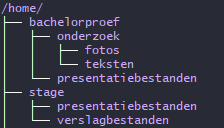
\includegraphics[width=0.45\textwidth]{img/mappenstructuur.png}}
    \caption{Mappen structuur basis configuraties.}
    \label{fig:mappen}
\end{figure}
\subsection{Opstellen cloud-init config bestand}
Als eerste zal het cloudconfig bestanden worden opgesteld. Dit bestand werd opgesteld met behulp van \autocite{clouddocs}.

Eerst werd er bekeken welke modules er nodig zullen zijn voor het opstellen van dit bestand. De modules \textit{packages} en \textit{package\_upgrade} zullen worden gebruikt voor de packages. De modules \textit{users} en \textit{groups} zullen worden gebruikt voor het toevoegen van gebruikers en groepen. 

Voor het toevoegen van de ssh sleutel, wordt de module \textit{ssh\_authorized\_keys} gebruikt. Hier worden de publieke sleutels die zijn toegelaten toegevoegd.

Voor het aanmaken van bestanden bestaat er de module \textit{write\_files}, spijtig genoeg is er geen module voor het aanmaken van mappen. Voor het aanmaken van de mapppenstructuur werd dus de module \textit{runcmd} gebruikt.

\subsubsection{Packages}
Hierna werd het effectieve bestand gevormd. Onder de \textit{packages} werden de 3 packages opgelijst: \textit{git}, \textit{pwgen} en \textit{tree}. Bij \textit{package\_upgrade} werd \textit{true} gezet. 
\begin{lstlisting}
packages:
    - pwgen
    - git
    - tree

package_upgrade: true
\end{lstlisting}

\subsubsection{Users \& Groups}
Bij \textit{groups} moest niet veel gedaan worden. Er werd gewoon de groepnaam van de groep gezet.

Bij \textit{users} werden veschillende dingen ingevuld. Eerst en vooral de name, \textit{bachelor}. Sudo werd op \textit{true} gezet zodat de gebruiker sudo rechten heeft. Bij groups de naam van de aangemaakte groep. Het wachtwoord onder passwd, proef, werd geëncypteerd met de tool: \autocite{toolmkpass}. Als shell werd ook voor \textit{/bin/bash} gekozen.
\begin{lstlisting}
groups:
    - test

users:
    - default
    - name: bachelor
    - passwd: 985b56433efe9898290b88d4dab853a2f09d7eb7a7b1b8d2cdd431
    - sudo: true
    - groups: test
    - shell: /bin/bash
\end{lstlisting}


\subsubsection{Runcdm}
Bij de module \textit{runcmd} werden alle commando's gezet voor het aanmaken van de mappen structuur. Dit zijn gewoon 5 \textit{mdkir} commando's. Dit is het commando voor het aanmaken van mappen.
\begin{lstlisting}
runcmd:
    - mkdir /home/bachelorproef/onderzoek/fotos
    - mkdir /home/bachelorproef/onderzoek/teksten
    - mkdir /home/bachelorproef/presentatiebestanden
    - mkdir /home/stage/presentatiebestanden
    - mkdir /home/stage/veslagbestanden
\end{lstlisting}

\subsubsection{Ssh}
Als laatste wordt de ssh sleutel toegevoegd aan de server. Bij de waarde \textit{<insert key value>} wordt de publieke sleutel van de host die gaat connecteren gezet.
\begin{lstlisting}
ssh_authorized_keys:
	- ssh-rsa <INSERT KEY VALUE>
\end{lstlisting}

Helemaal onderaan werd ook iets gezet onder de module \textit{final\_message}, namelijk: \textit{"The system is finally up, after \$UPTIME seconds"}. Door de waarde \textit{\$UPTIME} kan er gekeken worden hoelang de server nodig had om alles uit te voeren.

\subsection{Opstellen Ansible playbook}
Als tweede werd het Ansible playbook opgesteld. Als host wordt gekozen voor local-test en localhost, afhangend of het de lokale of cloud setup is. Aan het \textit{ansible.cfg} bestand werd ook nog de regel \textit{callback\_whitelist = profile\_tasks}. Zo kan er bekeken worden hoelang het draaien van het playbook duurde. Alle configuraties die worden gedaan werden in verschillende \textit{tasks} gezet. 

\subsubsection{Packages}
Voor het upgraden van de packages en installeren van de nodige packages werd de task \textit{apt} gebruikt.
\begin{lstlisting}
- name: Upgrade all packages to the latest version
  apt:
    name: "*"
    state: latest
- name: Install git
  apt:
    name: git
    state: present
- name: Install tree
  apt:
    name: tree
    state: present
- name: Install pwgen
  apt:
    name: pwgen
    state: present
\end{lstlisting}
\subsubsection{Mappen structuur}
Voor het aanmaken van de mappen structuur werd de task \textit{file} gebruikt. De state werd dan op directory gezet.
\begin{lstlisting}
- name: Creates direcory fotos
  file:
    path: /home/bachelorproef/onderzoek/fotos
    state: directory
- name: Creates direcory teksten
  file:
    path: /home/bachelorproef/onderzoek/teksten
    state: directory
- name: Creates direcory bachelor presentatie
  file:
    path: /home/bachelorproef/presentatiebestanden
    state: directory
- name: Creates direcory stage presentatie
  file:
    path: /home/stage/presentatiebestanden
    state: directory
- name: Creates direcory stage verslag
  file:
    path: /home/stage/verslagbestanden
    state: directory
\end{lstlisting}
\subsubsection{Users \& groups}
Bij het aanmaken van de gebruikers en groepen werden de tasks \textit{group} en \textit{user} gebruikt. Bij de \textit{user} werden het shell en password meegeven. Ook de groups werden meegegeven waaronder de adin group zodat de user sudo rechten heeft.
\begin{lstlisting}
- name:  add group test
  group:
    name: test
    state: present
- name:  add user bachelor
  user:
    name: bachelor
    groups: test,admin
    shell: /bin/bash
    password: 985b56433efe9898290b88d4dab853a2f09d7eb7a7b1b8d2cdd431e2920c35
\end{lstlisting}

\subsubsection{Ssh}
Voor het toevoegen van de ssh sleutel aan de server, zodat er een extra connectie kan worden gelegd, wordt de task \textit{authorized\_key} gebruikt. Voor de lokale setup wordt dit via een bestand gedaan in de gedeelde map vagrant. Voor de cloud setup wordt dit opgehaald via git.
\begin{lstlisting}
- name: Set authorized key taken from file
  authorized_key:
	user: charlie
	state: present
	key: "{{ lookup('file', '/vagrant/key') }}"
	
- name: Set authorized key taken from file
  authorized_key:
	user: charlie
	state: present
	key: http://www.github.com/path-to-key
\end{lstlisting}

\subsection{Ansible \& cloud-init omgevingen}
Beide bestanden die apart gemaakt zijn, zijn vrij complexloos. Beide bestanden zijn vrij duidelijk. Wat als nadeel is voor het gebruik van een combinatie van Ansible en cloud-init. De enige uitvoering die complex is de bestanden is het aanmaken van de mappen via cloud-init. Dit is een beetje 'dirty' gedaan. Voor het werken met een combinatie gaat eerst alles via cloud-init worden gedaan. Het aanmaken van de mappen dan via Ansible.

\subsubsection{Verwijzig Anisble lokaal}
De verwijzing naar Ansible in de lokale setup zal gebeuren via de module \textit{write\_files}. Met de tool \autocite{toolbas64} werd de het playbook geëncodeerd. Hieronder is het playbook dat wordt geëncodeerd.
\begin{lstlisting}
- hosts: localhost
  tasks:
	- name: Creates direcory fotos
	  file:
		path: /home/bachelorproef/onderzoek/fotos
		state: directory
	- name: Creates direcory teksten
	  file:
		path: /home/bachelorproef/onderzoek/teksten
		state: directory
	- name: Creates direcory stage presentatie
	  file:
		path: /home/bachelorproef/presentatiebestanden
		state: directory
	- name: Creates direcory bachelor presentatie
	  file:
		path: /home/stage/presentatiebestanden
		state: directory
	- name: Creates direcory stage verslag
	 file:
		path: /home/bachelorproef/stage/verslagbestanden
		state: directory
\end{lstlisting}

In cloud-init wordt in de module \textit{write\_files} het bestand aangemaakt. In de module \textit{runcmd} wordt dan het playbook aangeroepen met een commando.
\begin{lstlisting}
write_files:
	- path: "/home/ansible/playbook.yaml"
	encoding: "b64"
	content: Ci0gaG9zdHM6IGxvY2FsaG9zdAogIHRhc2tzOgogICAgLSBuYW1lOiBDcmVhdGVzIGR
runcmd:
	- ansible-playbook -i, /home/ansible/playbook.yaml
\end{lstlisting}

\subsubsection{Verwijzing Ansible cloud}
Voor de cloud setup wordt de verwijzing via github gedaan. Er wordt een git repository aangemaakt met het playbook in. Die wordt dan gecloned in cloud-init en uitgevoerd.

In cloud-init wordt drie modules toegevoegd: \textit{runcmd}, \textit{no\_ssh\_fingerprints} en \textit{ssh\_keys}. In de module \textit{ssh\_keys} wordt de private sleutel toegevoegd connectie legt met de git repo. In de module \textit{runcmd} worden 2 commando's gezet: de git clone en het uitvoeren van het playbook. \textit{no\_ssh\_fingerprints} wordt op true gezet. Zo geeft het geen error dat de server de host niet kent.
\begin{lstlisting}
ssh_keys:
	rsa_private: | <key>
no_ssh_fingerprints: true
runcmd:
	- ssh-agent bash -c 'ssh-add /etc/ssh/ssh\_host\_rsa\_key; 
	  git clone <repo>'
	- ansible-playbook -i, /home/ansible/playbook.yaml
\end{lstlisting}

\section{Uitvoering \& resultaten}

\subsection{Lokaal}

\begin{table}[!htb]
    \centering
    \begin{tabular}{| l | l | l |}
        \hline
         & \textbf{Uitvoeringstijd} & \textbf{Aantal lijnen code}  \\ \hline
        cloud-init & 0 sec & 24 \\ \hline
        Anisble & 0 sec & 53 \\ \hline
        cloud-init \& Ansible & 0 sec & 0 \\
        \hline
    \end{tabular}
	\caption{Resulaten tabel van Basisconfiguraties op de lokale servers.}
    \label{tab:tabel lokale resultaten basis}
\end{table}



\subsection{Cloud}

\begin{table}[!htb]
    \centering
    \begin{tabular}{| l | l | l |}
        \hline
        & \textbf{Uitvoeringstijd} & \textbf{Aantal lijnen code}  \\ \hline
        cloud-init & 0 sec & 0 \\ \hline
        Anisble & 0 sec & 53 \\ \hline
        cloud-init \& Ansible & 0 sec & 0 \\
        \hline
    \end{tabular}
    \caption{Resulaten tabel van Basisconfiguraties op de cloud servers.}
    \label{tab:tabel cloud resultaten basis}
\end{table}

Meerdere server bekijen bij cloud